% Sebastián Petrík MIP ZS 2020/2021
% FIIT STU BA
% Primarny kompilator: latexmk, MikTex

\documentclass[10pt,slovak,a4paper]{article}
\usepackage[slovak]{babel}
\usepackage[utf8]{inputenc}
\usepackage{graphicx}
\usepackage{url}
\usepackage{cite}
\usepackage{indentfirst}
\usepackage{multicol}
\usepackage[unicode]{hyperref}
\usepackage{csquotes}
\usepackage{caption}
\usepackage{array}

\pagestyle{headings}
\title{Časový manažment a organizácia informácií\thanks{Semestrálny projekt v predmete Metódy inžinierskej práce, ak. rok 2020/21, vedenie: Zuzana Špitálová}}
\author{Sebastián Petrík\\[2pt]
	{\small Slovenská technická univerzita v Bratislave}\\
	{\small Fakulta informatiky a informačných technológií}\\
	{\small \texttt{xpetriks1@stuba.sk}}
	}
\date{\small 8. december 2020}

\begin{document}
\maketitle

\begin{abstract}
Svojím článkom by som sa chcel zamerať na problematiku časového manažmentu (time management) a plánovania úloh ako súčasť individuálnej a skupinovej organizácie informácií. Plánujem preskúmať základné znaky tejto disciplíny, jej rôzne aspekty, výhody, nevýhody a dôležitosť pre rôzne skupiny ľudí. Budem sa venovať zhodnoteniu aktuálneho stavu výskumu v tejto oblasti.

Ďalej preskúmam možnosti nástrojov spojených s organizáciou času a informácií (digitálne aj klasické), ich kategórie, rozdielne aj podobné vlastnosti. Chcem opísať aktuálny stav digitálnych nástrojov na organizáciu času, spôsoby, akými ich ľudia využívajú a kategórie používateľov týchto nástrojov. Zároveň by som rád preskúmal vplyv časového manažmentu v edukačnom prostredí (vplyv na študenta vysokej školy, jeho produktívnosť a psychiku).

\end{abstract}
\newpage

\section{Úvod}

	Časový manažment, plánovanie úloh a organizácia informácií sú pojmy, s ktorými sa často stretne človek prakticky v každej oblasti. Týkajú sa nielen pracovníkov vo firme (vykonávajúcich či už psychickú, ale aj fyzickú prácu), ale aj hlavne študentov vysokých a stredných škôl.
	
	Človek je v dnešnom svete zahltený množstvom informácií a úlohami, ktoré je potrebné vykonať v určitom časovom intervale. Prirodzene preto vzniká potreba vytvoriť si určitý systém organizácie.
	
	Cieľom je nielen zabezpečiť dokončenie úloh v termíne, ale aj do určitého stupňa eliminovať zábudlivosť, centralizovať dôležité informácie a termíny, zlepšiť kvalitu práce, zvýšiť efektivitu a zbaviť sa zbytočného stresu.
	
\section{Stav v oblasti}

	Napriek tomu, že najmä v pracovných prostrediach pracujúcich s informáciami sú pocity uponáhľanosti a prerušenia súvislej práce vplyvom určitých vyrušení (tzv. fragmentácia práce \cite{NoTask}) pomerne časté a veľmi rozšírené, existuje prekvapivo malé množstvo akademického výskumu venujúceho sa manažmentu a plánovaniu úloh \cite{Franssila}. 
	
	Väčšina štúdií v tomto obore \cite{Franssila,NoTask,Blandford} sa venuje práve fragmentácii práce a analýze pracovných prostredí a praktík časového manažmentu, ktoré tieto prostredia využívajú.
	
	Niektoré štúdie \cite{Franssila, Blandford, Haraty} však skúmajú nástroje, ktoré je možné využiť na organizáciu času a úloh. Taktiež sa venujú kategorizácii používateľov podľa nimi rôznych preferovaných spôsobov organizácie úloh, ale aj dôsledok existencie rôznych kategórií používateľov na dizajn nástrojov určených pre tento problém \cite{Haraty}.
	
	Tento problém je zároveň pomerne dôležitý v edukačnom prostredí. Niektoré psychologické štúdie \cite{Macan} sa venujú vplyvu časového manažmentu na študentov a ich psychiku.
	
\section{Problematika}

	S problematikou časového manažmentu sa dajú spojiť rôzne pojmy:
	\begin{itemize}
		\item časový manažment
		\item plánovanie úloh
		\item organizácia informácií
		\item fragmentácia práce
	\end{itemize}

	Franssila vo svojej štúdii\cite{Franssila} vysvetľuje, že koncepty úlohového manažmentu, plánovania úloh, plánovania aktivít a časového manažmentu sú často v akademickej literatúre využívané ako synonymá, referujúce na rôzne kategórie aktivít spojených s plánovaním a načasovaním úloh\cite{Franssila}.
	
	Je dôležité si uvedomiť, že tieto rôzne pojmy sa venujú spoločnému problému, a preto sú často využívané spolu. Tento fakt si môžeme všimnúť napríklad pri skúmaní funkcionality nástrojov spojených s touto problematikou, kde v jednom nástroji často nachádzame funkcie pre správu času, ale aj organizáciu úloh a informácií spojených s týmito úlohami.
	
	\paragraph{}
	\begin{figure*}[tbh]
		\centering
		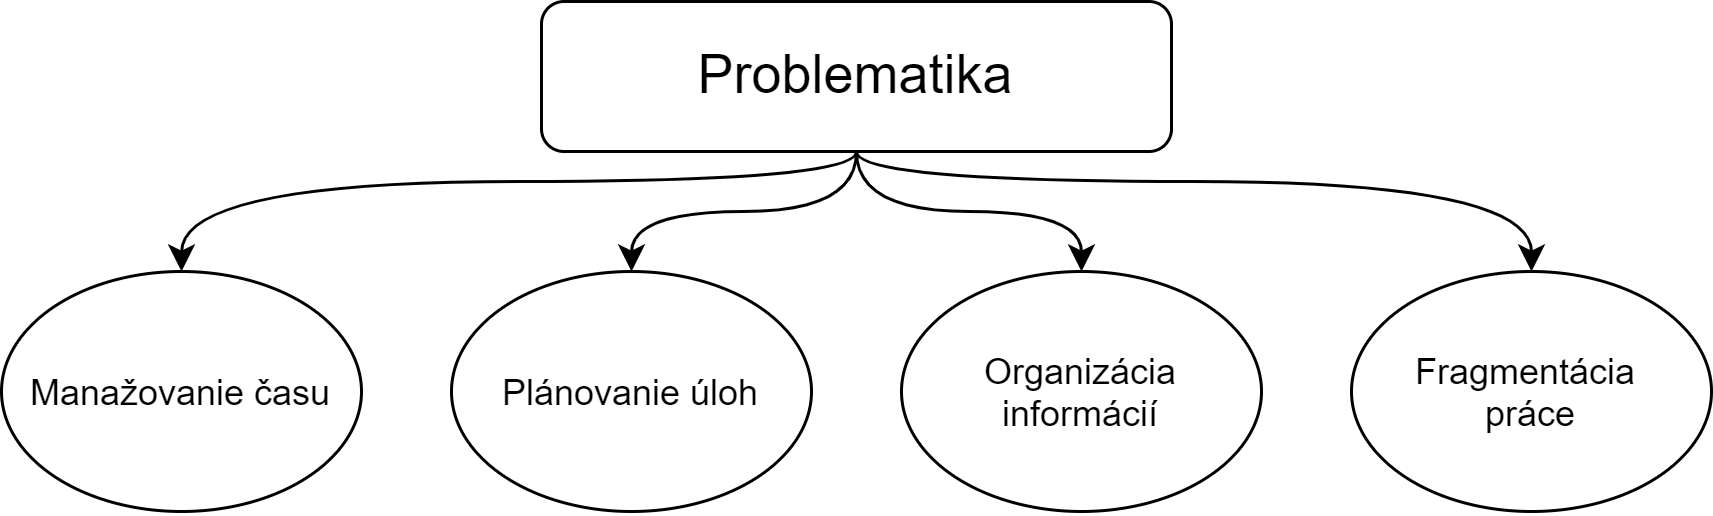
\includegraphics[width=0.9\textwidth]{problematika.png}
	\caption{Pojmy časového manažmentu}
	\label{f:pojmy}
	\end{figure*}
	
	\subsection{Časový manažment} \label{casovy_manazment}
	
		Časový manažment by sme mohli definovať ako súbor aktivít spojených s organizáciou času, ktorý má individuál alebo skupina prístupný v určitom časovom intervale.
		
		Tento časový interval môže byť vnímaný z rôzneho hľadiska - môže byť vymedzený napr. základnými potrebami (spánok, stravovanie), určitými termínmi (napr. potreba dokončiť projekt do termínu - vzniká potreba manažovať si tento vymedzený čas), a pod.
		
	\subsection{Plánovanie úloh}
	
		Plánovanie úloh je možné vnímať ako priamu súčasť časového manažmentu, teda ako konkrétne dedikovanie jednotlivých časových segmentov z určeného časového intervalu na riešenie určitých úloh.
		
		Franssila uvádza, že hlavné aktivity spojené s plánovaním úloh sú \cite{Franssila}:
		\begin{itemize}
			\item plánovanie
			\item prioritizácia
			\item tvorba zoznamov
		\end{itemize}
		
		Taktiež vysvetľuje, že s plánovaním úloh sú spojené rôzne výzvy, konkrétne integrácia rôznych médií, preusporiadanie úloh (napr. vplyvom nečakaných udalostí), zisťovanie vhodnosti konkrétnej úlohy, identifikovanie vhodných časových intervalov, tvorba flexibilných časových plánov, manažovanie dlhodobých cieľov, odhad trvania konkrétnej úlohy a identifikovanie pôvodu rozličných úloh\cite{Franssila}.
		
		Keď sa pozrieme priamo na vykonávanie daných úloh, je možné si všimnúť dalšie ťažkosti, s ktorými sa človek stretne - dokončenie náročných úloh, splnenie už naplánovaných úloh, splnenie dlhodobých cieľov, splnenie úloh nezahŕňajúcich iných ľudí, pamätanie si malých úloh, udržiavanie dostatočnej motivácie a zhodnotenie dosiahnutých úspechov\cite{Franssila}.
		
		Môže nám dobrý časový manažment pomôcť pri prekonávaní týchto výziev a ťažkostí? Môžeme zhodnotiť, že určite áno, no je potrebné si uvedomiť, že to nemusí stačiť.
		
		Dôležitou podmienkou pre správny časový manažment je prirodzene správna sebadisciplína. Dalo by sa povedať, že tieto dve vlastnosti človeka sú v určitej symbióze a práca na zlepšení časového manažmentu individuála môže mať kladný vplyv na jeho sebadisciplínu a naopak.
		
	\subsection{Organizácia informácií}
	
		S časovým manažmentom a plánovaním úloh je často spojená aj všeobecná organizácia informácií. Už samotné termíny je potrebné určitým spôsobom organizovať, no pri plánovaní úloh sa stretávame aj s inými typmi informácí, ako napr. kontakty, adresy, emailové adresy, rôzne odkazy, zoznamy, poznámky a pod.
	
	\subsection{Fragmentácia práce}
	% definicia
		Jedným z dôsledkov nedostatočného časového manažmentu môže byť práve vysoká fragmentácia práce.
		
		Môžeme ju definovať ako prerušenie súvislej pracovnej aktivity. Rôzne štúdie spomínajú, ako ľudia pracujúci s informáciami často dedikujú malé množstvá času určitým aktivitám a často menia činnosti. Takéto správanie bolo zaznamenané napr. pri manažéroch, finančných analytikoch a softvérových vývojároch\cite{NoTask}.
		
		Štúdia\cite{NoTask} uvádza, že fragmentácia p. má dva hlavné aspekty - dĺžka času využitá na súvislú aktivitu a prerušenia danej aktivity. Práca dosahuje tým väčšiu fragmentáciu, čím menej času človek využije na plnenie úlohy a čím viac je človek vyrušovaný. Je síce pravda, že striedanie úloh môže mať určité výhody - môže nám to pomôcť oddýchnuť si a získať nové nápady. Na druhej strane, striedanie aktivít môže zhoršiť koncentráciu na jednotlivé úlohy a môže znížiť efektivitu a množstvo vykonanej práce\cite{NoTask}.
		
		Fransilla zároveň uvádza, že ľudia pracujúci s informáciami pociťujú fragmentáciu práce najčastejšie vo forme uponáhľanosti a zábudlivosti \cite{Franssila}.
		
	\subsection{Vyrušenia}
	% typy, mozu byt benefitial, inkubacia problemu
	% 
		Vyrušenia sú jedným s hlavných faktorov pri skúmaní fragmentácie práce. Individuál pre ne často preruší aktivitu a pokračuje v nej až po určitom čase.
		
		Štúdia \cite{NoTask} uvádza dva základné typy vyrušení - externé a interné.
		
		Externé vyrušenia pochádzajú z vonkajšieho prostredia, napr. zazvonenie telefónu, príchod kolegu do kancelárie, nový email alebo správa \cite{NoTask}.
		
		Interné vyrušenia naopak vznikajú práve vtedy, keď individuál preruší svoju aktivitu voliteľne. Môže napr. potrebovať prestávku, alebo si premyslieť určitú myšlienku \cite{NoTask}. Fransilla uvádza, že práve tieto vyrušenia (spôsobené vlastnou vôľou) sú najčastejšie \cite{Franssila}.
		
		Vyrušenia majú zároveň rôzne priority\cite{NoTask}, a preto je dôležité správne prioritizovať aj ne - niektoré sú nevyhnutné, no niektoré sú často zbytočné a mali by sme sa ich vyvarovať.

\section{Nástroje na organizáciu času a informácií}
	% Fransilla introduction~interface design
		Organizácia času a informácií určite nie je triviálna záležitosť. Je to komplexná aktivita (časť~\ref{casovy_manazment}), a preto tu vzniká potreba určitých nástrojov, ktoré by to človeku uľahčili.
		
		Dali by sa rozdeliť na dve základné kategórie:
		\begin{itemize}
			\item klasické,
			\item digitálne.
		\end{itemize}
		
	\subsection{Klasické}
		Medzi klasické nástroje môžeme zaradiť nástroje, ktoré nie sú úzko spojené s modernou dobou počítačov a elektroniky. Môžu to byť napríklad:
		\begin{itemize}
			\item pero a papier, jednoduchý zošit
			\item diár
			\item kalendár
			\item nástenka a nalepovacie bloky
		\end{itemize}
	
	\subsection{Digitálne}
		Na rozdiel od klasických nástrojov, tie digitálne sú často práve určité počítačové programy, alebo elektronické zariadenia. Sú to napríklad :
		\begin{itemize}
			\item PDA (Personal Digital Assistant)
			\item Poznámkový tablet
			\item Skupina programov Microsoft Office (napr. MS Word, MS Outlook, MS Excel, a iné)
			\item Google Keep
			\item Notion
			\item Evernote
		\end{itemize}
		
		Je dôležité si uvedomiť, že trh aplikácií pre časový manažment sa neustále rozvíja. Existuje ich mnoho a individuál by mal pri vyberaní takého nástroja určite vyskúšať viacero z nich, pretože mu niektoré nástroje môžu vyhovovať viac, ako iné. Existujú aj určité stránky \cite{JustinPot9best}, ktoré odporúčajú takéto produkty, no je potrebné si uvedomiť, že sú prevažne subjektívne.
		
	\subsection{Kategórie používateľov}
		
		Typickým znakom digitálnych nástrojov je veľké množstvo rozličných funkcií. Je to práve ponuka funkcií, v čom sa rôzne dostupné produkty líšia.
	
		Štúdia \cite{Haraty} uvádza, že používateľov nástrojov by sme mohli rozdeliť do určitých kategórií v závislosti na tom, aké nástroje (a teda aké funkcie) používajú:
		
		\par
		\begin{itemize}
			\item \textbf{Adopters} - využívajú dedikovaný nástroj,
			\item \textbf{DIYers} (\enquote{do-it-yourself-ers}) - využívajú všeobecné nástroje (MS word, diár), vytvárajú si vlastný systém (čoho dôvodom môžu byť nepostačujúce existujúce nástroje alebo napr. potreba personalizácie),
			\item \textbf{Make-doers} - minimálne využitie nástrojov (email, pero a papier, MS Word), preferujú predvolené nastavenia, využívajú minimálne funkcie časového manažmentu \cite{Haraty}.
		\end{itemize}
		
		Na základe tohto rozdelenia bol uskutočnený touto štúdiou prieskum medzi 19 účastníkmi ohľadom nástroja, ktorý využívajú \cite{Haraty}:
		
		\par
		\begin{table}[tbh]
			
			\begin{center}
				\begin{tabular}{ | p{0.12\linewidth} | p{0.60\linewidth} | p{0.20\linewidth} | }
					\hline
						\textbf{č. účastníka} & \textbf{Nástroj} & \textbf{Kategória} \\ \hline
						1 & Papierový diár & DYIer \\ \hline
						2 & Kúsky papiera, Notepad, email & DYIer \\ \hline
						3 & Papier, email, alarm & DYIer \\ \hline
						4 & Word dokument, Google Calendar, poznámkový zošit, alarm & DYIer \\ \hline
						5 & OneNote, Outlook & DYIer \\ \hline
						6 & Papier & DYIer \\ \hline
						7 & Word dokument, Google Calendar & DYIer \\ \hline
						8 & Microsoft Excel, Word, Google Calendar/ Tasks, iPhone calendar & DYIer \\ \hline
						9 & Papier, kalendáry & DYIer \\ \hline
						10 & Wiki, poznámkový zošit, sticky notes & DYIer \\ \hline
						11 & Word dokument, papierový zošit & DYIer \\ \hline
						12 & AbstractSpoon, Email(Gmail), Google Calendar & Adopter \\ \hline
						13 & Things, Google Calendar & Adopter \\ \hline
						14 & Google Tasks, Email, Google Calendar, Whiteboard, wiki & Adopter \\ \hline
						15 & OmniFocus, kolaboratívny email & Adopter \\ \hline
						16 & papierový poznámkový blok, iPod calendar & Make-doer \\ \hline
						17 & Email, Google Calendar & Make-doer \\ \hline
						18 & Calendar (Google, iphone), poznámkový zošit & Make-doer \\ \hline
						19 & Google Calendar, Firefox Tabs, textové súbory & Make-doer \\ \hline
				\end{tabular}
				\caption{Nástroje využívané účastníkmi prieskumu \cite{Haraty}}
			\end{center}
		\end{table}
		
		\paragraph{}
		\begin{figure*}[tbh]
			\centering
			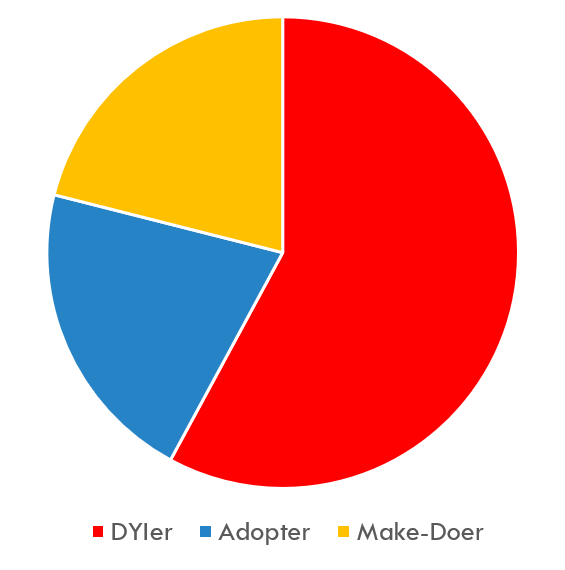
\includegraphics[width=0.6\textwidth]{grafkateg.png}
		\caption{Pomer kategórií používateľov z prieskumu \cite{Haraty}}
		\label{f:kategraf}
		\end{figure*}
		
		Podľa diagramu (Obr. \ref{f:kategraf}) si môžeme všimnúť, že najpočetnejšou kategóriou sú práve používatelia, ktorí si vytvárajú vlastný systém a preferujú personalizáciu. Tento fakt by mohol byť dôležitý pre budúci vývoj nástrojov časového manažmentu - nástroje by mali byť ľahko prispôsobiteľné používateľom.
		
\section{Vplyv a dôležitosť časového manažmentu}

		Časový manažment má veľký vplyv na prakticky každú pracovnú sféru, či už vo firmách, alebo aj v edukačnom prostredí. Hlavnými výhodami dobrého časového manažmentu môže byť práve menej stresu, lepšia efektivita práce (a teda viac voľného času) a lepšie výsledky.
		
	\subsection{Vplyv na psychiku a stres}
	
		Vplyvu časového manažmentu na človeka a jeho psychiku sa venujú rôzne psychologické štúdie \cite{Macan}.
	
		Je bežné, že študent vysokej školy vníma svoje štúdium ako veľmi stresujúce.Fransilla zároveň uvádza, že ľudia pracujúci s informáciami pociťujú fragmentáciu práce najčastejšie vo forme uponáhľanosti a zábudlivosti \cite{Franssila}.
		
		Macan \cite{Macan} vo svojej štúdii uvádza, že existujú rôzne faktory, ktorými môžeme hodnotiť efekt časového manažmentu na človeka. Jedným  z týchto faktorov je napríklad schopnosť vnímať svoju kontrolu nad vlastným časom. Študenti v prieskume \cite{Macan}, ktorí mali túto schopnosť preukázali značne lepšie výsledky, lepšiu celkovú spokojnosť z práce a života, menej prepracovanosti a menej pocitov napätia \cite{Macan}.
		
	\subsection{Spojitosť s inými odbormi}
		
		\paragraph{Spoločenské súvislosti.}
		
		\paragraph{Historické súvislosti.}
		\paragraph{Technológia a ľudia.}
		\paragraph{Udržateľnosť a etika.}
		
		
\section{Záver}

\bibliography{literatura}
\bibliographystyle{plain}
\end{document}
